% Copyright 2004 by Till Tantau <tantau@users.sourceforge.net>.
%
% In principle, this file can be redistributed and/or modified under
% the terms of the GNU Public License, version 2.
%
% However, this file is supposed to be a template to be modified
% for your own needs. For this reason, if you use this file as a
% template and not specifically distribute it as part of a another
% package/program, I grant the extra permission to freely copy and
% modify this file as you see fit and even to delete this copyright
% notice. 

\documentclass{beamer}
\usepackage{amsmath}
\usepackage{bm}
\usefonttheme{professionalfonts}
\usepackage{newtxtext,newtxmath}
\usepackage{ragged2e}
\newcommand{\bh}{\bm{h}}
\newcommand{\bt}{\pmb{\theta}}
\newcommand{\bG}{\pmb{\Gamma}}
\newcommand{\p}{\pause}
\newcommand{\pitem}{\pause \item}
\newcommand{\N}{\mathcal{N}}
\newcommand{\Y}{\bm{\mathcal{Y}}}
% There are many different themes available for Beamer. A comprehensive
% list with examples is given here:
% http://deic.uab.es/~iblanes/beamer_gallery/index_by_theme.html
% You can uncomment the themes below if you would like to use a different
% one:
%\usetheme{lankton-keynote}
%\usetheme{AnnArbor}
%\usetheme{Antibes}
%\usetheme{Bergen}
%\usetheme{Berkeley}
%\usetheme{Berlin}
%\usetheme{Boadilla}
%\usetheme{boxes}
%\usetheme{CambridgeUS}
%\usetheme{Copenhagen}
%\usetheme{Darmstadt}
%\usetheme{default}
%\usetheme{Frankfurt}
%\usetheme{Goettingen}
%\usetheme{Hannover}
%\usetheme{Ilmenau}
%\usetheme{JuanLesPins}
%\usetheme{Luebeck}
\usetheme{Madrid}
\usepackage[final]{pdfpages}
%\usetheme{Malmoe}
%\usetheme{Marburg}
%\usetheme{Montpellier}
%\usetheme{PaloAlto}
%\usetheme{Pittsburgh}
%\usetheme{Rochester}
%\usetheme{Singapore}
%\usetheme{Szeged}
%\usetheme{Warsaw}
%\usecolortheme{beetle}

\newcommand*\samethanks[1][\value{footnote}]{\footnotemark[#1]}

\setbeamertemplate{navigation symbols}{}%remove navigation symbols
\title[The Network of FDI Flows]{The Network of Foreign Direct Investment Flows:\\Theory and Empirical Analysis\thanks{\scriptsize {Acknowledgement: This material is based on work supported by the National Science Foundation under IGERT Grant DGE-1144860, Big Data Social Science.}}}


\author[Schoeneman, Zhu, \& Desmarais]{%
  \texorpdfstring{%
    \begin{columns}
      \column{.3\linewidth}
      \centering
      John Schoeneman{\thanks{\scriptsize{Pennsylvania State University}}} \\ \scriptsize{jbs5686@psu.edu\\ PhD Candidate}
      \column{.3\linewidth}
      \centering
      Boliang Zhu{\samethanks[2]} \\ \scriptsize{bxz14@psu.edu\\ Assistant Professor}
    \end{columns}
    \vspace{12pt}
    \begin{columns}
      \column{.3\linewidth}
      \centering
      Bruce Desmarais{\samethanks[2]}\\ \scriptsize{bdesmarais@psu.edu\\ Associate Professor}
    \end{columns}
 }
 {Author 1, Author 2, Author 3}
}

\date{April 8, 2017}



% - Use the \inst command only if there are several affiliations.
% - Keep it simple, no one is interested in your street address.

% - Either use conference name or its abbreviation.
% - Not really informative to the audience, more for people (including
%   yourself) who are reading the slides online


% This is only inserted into the PDF information catalog. Can be left
% out. 

% If you have a file called "university-logo-filename.xxx", where xxx
% is a graphic format that can be processed by latex or pdflatex,
% resp., then you can add a logo as follows:

% \pgfdeclareimage[height=0.5cm]{university-logo}{university-logo-filename}
% \logo{\pgfuseimage{university-logo}}



\begin{document}

\begin{frame}
  \titlepage
  %Slide 1
%?Good afternoon and thank you for the opportunity to present this paper today on FDI networks. My name is John Schoeneman and I am currently a PhD candidate at Penn State. My coauthors, Dr. Zhu and Dr. Desmarais, are both professors at Penn State.?  
\end{frame}




\begin{frame}{Introduction}


\begin{itemize}
 \item{Motivation}
 \begin{itemize}
\item{Violation of Independence Assumptions}
\item{Theoretical Importance of Dependence Terms}
 \end{itemize}
\item{FDI as a Network}
\begin{itemize}
\item{Reciprocity}
\item{Transitivity}
 \end{itemize}

  \item{Simultaneously test exogenous variables}
 \end{itemize}

  %Slide 2
% Foreign Direct Investment has grown over the years in magnitude and the number of destinations as well as senders, creating an intricate web of relationships for both trade and investment. Alongside of this increase, scholars have sought to explain who sends FDI and who receives it with a number of economic and political variables.  Historically, statistical models that have been used to test theories rely on the assumption that countries and pairs of countries are independent of one another. We argue that for most  foreign direct investment flows, and most applications, that this assumption is overly optimistic. This lack of independence though is not our only motivator to study the network of FDI. We argue that dependence terms such as reciprocity and clustering are theoretically important as well and present hypotheses for them. Furthermore, we test these network terms simultaneously with a selection of exogenous variables that have been found to be important in the literature. 


\end{frame}




\begin{frame}{Reciprocity}

\begin{itemize}
\item{Reciprocity}\\

\centering{
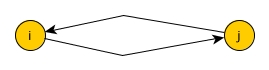
\includegraphics[scale=.7, clip=true, trim=0cm 0cm 0cm 0cm]{slides_figures/reciprocity.jpg}
}\\

\justifying
\item{Standard practice to resolve political opposition from competing firms}\\
\item{Anti-reciprocal relationship in mixed dyads}

\end{itemize}


  %Slide 3
% We focus on two network dependencies in our model and provide theoretical reasoning for them. The first is reciprocity, also known as mutuality. For the FDI network, this statistic is higher when the more FDI country i sends to country j, the more likely country j is to send more FDI to country i. As with trade, expansion of foreign firms into a country's market is generally met with some opposition by the owners of similar firms. The political route to resolve this conflict is through reciprocal agreements. This allows politicians to build up sufficient support to remove barriers for FDI by granting the opposing firms or other sectors of the economy access to new markets.


\end{frame}

\begin{frame}{Transitivity}

\begin{itemize}
\item{Transitivity}

\centering{
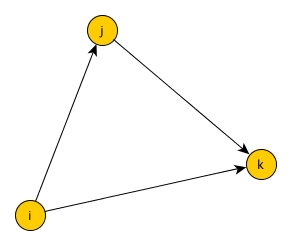
\includegraphics[scale=.5, clip=true, trim=0cm 0cm 0cm 0cm]{slides_figures/transitivity.jpg}
}\\
\justifying
\item{MNC expansion and supply-chain fragmentation}
\item{Risk of Expropriation}
\item{PTA networks}

\end{itemize}
  %Slide 4
% The second network dependency we estimate is transitivity, also known as the clustering coefficient. The transitivity network statistic is a triadic closure that is not a loop. Put another way, the stronger the two-path between country i and j, the higher the likelihood is of a stronger tie between i and j. Global production supply chains are increasingly complex and disaggregated. With large MNCs being the dominant players in global trade networks, they often invest in multiple countries, even for only one type of finished product, and are increasingly involved in all levels of production. This behavior increases the chance that an investor is more likely to invest in a country for which a two-path already exists. Also, since there is inherent risk in investment, the possibility of expropriation of fixed investments, investment is encouraged to cluster along particular countries that have a sustained interest in protecting investors, which also leads to triadic closures in the network. Another key factor is that much of FDI is vertical and thus dependent on trade liberalization. Preferential trade agreements can reinforce or expand these clusters through the expansion and liberalization of trade networks. 


\end{frame}



\begin{frame}{FDI Data and Exogenous Covariates}

\begin{itemize}
\item{Bilateral FDI statistics from UNCTAD, 2001-2012}
\end{itemize}

\begin{columns}[T]
    \begin{column}{.5\textwidth}
\begin{itemize}
\item{Dyad-level Covariates}
\begin{itemize}
\footnotesize{
\item{Gravity +} 
\item{Contiguity +} 
\item{Common Language +} 
\item{Four Types of Defense Treaties +}  
\item{Colonial Relationships +}
 \item{PTA depth +}
 }
\end{itemize}
\end{itemize}
    \end{column}
    \begin{column}{.5\textwidth}
\begin{itemize}
\item{Node-level Covariates (s/r)}
\begin{itemize}
\footnotesize{
\item{GDP per capita +/-} 
\item{GDP Growth Rate +/+} 
\item {Polity IV +/+} 
\item{Political Violence -/-} 
\item{Trade Openness +/+}
 }
\end{itemize}
\end{itemize}
        \end{column}
  \end{columns}
 
%Slide 5
 %Our dependent variable is from recently made available data by UNCTAD. It covers 2001 to 2012. We use FDI stock levels since we take the log and FDI stock has fewer negative values that need to be converted to zeros. Although, we include a lagged dependent variable, so our covariates are estimating remaining variation, which is FDI flows.  
 
 % We include a number of dyadic and node level covariates in the model that have been commonly used in the literature. They are listed below with their expected relationship. Node level covariates are included in the model both for sending nodes and receiving node.
  

\end{frame}




\begin{frame}{The Exponential Random Graph Model (ERGM)}

The probability (likelihood function) of observing the network is:

$$ \text{Pr}_{\bm{\theta};h;\bm{g}}( \bm{Y}=\bm{y} )=\frac{ h(\bm{y})\text{exp}( \bm{\theta} \cdot \bm{g} (\bm{y}) )}{\bm{\kappa}_{h,\bm{g}}(\bm{\theta})} $$


Decomposition:
$$
\underbrace{\bm{h(y)}}_{Distribution} \qquad \underbrace{\bt}_{Effects} \qquad \underbrace{\bm{g(y)}}_{Net\hspace{3pt} Stats} \qquad \underbrace{\bm{\kappa}_{h,\bm{g}}(\bm{\theta})} _{Normalizer}
$$

%Slide 6
% We use the  count exponential random graph model (ERGM) for estimating the network dependencies and exogenous covariates The exponential random graph model MLE is approximated using MCMC because of computation limitations and the intractability of the normalizing constant, kappa. The Poisson reference function is used to parameterize the components of our model that are edge-specific, noted as h(y). Theta is the exogenous covariates and g(y) includes the network statistics.


\end{frame}

\begin{frame}{ERGM Constants}

$$\text{Sum}:\bm{g(y)} = \sum_{(i,j) {\in} \mathbb{Y}}\bm{y}_{i,j}$$

$$\text{Sum, Fractional Moment}:\bm{g(y)} = \sum_{(i,j) {\in} \mathbb{Y}}\bm{y}_{i,j}^{1/2}$$

$$\text{Non-Zero}: \bm{g}_k = \sum_{(i,j) {\in} \mathbb{Y}} \mathbb{I}(\bm{y}_{i,j} \neq 0)$$
%Slide 7
%For this model we use both the sum of edges and the fractional moment of edges. The first here is analogous to an intercept term, which is the sum of all edges and the fractional moment is a variance stabilizer. The non-zero term allows us to account for zero-inflation, here roughly 80% of the possible edges, by having non-zero values be distributed conditional on not being zero. This modifies the top equation by taking the product of two different thetas, one for non-zero values and another for the entire graph. 

\end{frame}

\begin{frame}{ERGM Dependence Terms}
$$ \text{Reciprocity}: \bm{g(y)} = \sum_{(i,j) {\in} \mathbb{Y}}min(\bm{y}_{i,j},\bm{y}_{j,i})$$

$$\text{Transitive Weights}: \bm{g(y)} =  \sum_{(i,j) {\in} \mathbb{Y}}\min\bigg( \bm{y}_{i,j}, \max\limits_{k{\in}N}\Big(\min(\bm{y}_{i,k},\bm{y}_{k,j})\Big) \bigg),$$ 
%Slide 8
% Reciprocity is estimated as the minimum of the dyad, which is that the conditional probability for a particular value of  Yij is deflated by the theta for mutuality for every unit by which Yi,j is less than Yj,i. Or put differently, larger minimum values increase the value of reciprocation. 

% This specification for transitive weights measures weakest two-path between nodes i and j. The statistic is then the sum over the dyads (i, j) of the  strongest two-path from i to j where the strength of the two-path is measured by the minimum edge value in the two-path. Here the effect can be interpreted as the stronger the two-path, the higher the FDI from i to j and conversely the more FDI there is from i to j, the stronger the two-path (Krivitsky 2011)

\end{frame}

\begin{frame}{ERGM Covariates}

$$ \text{Dyadic Covariate}: \bm{g(y,x)} = \sum_{(i,j)} \bm{y}_{i,j}x_{i,j}$$ 

$$ \text{Sender Covariate}: \bm{g(y,x)} = \sum_{i}x_i \sum_{j} \bm{y}_{i,j}$$

$$ \text{Receiver Covariate}: \bm{g(y,x)} = \sum_{j}x_j \sum_{i} \bm{y}_{i,j}$$
%Slide 9
% Dyadic covariates are estimated by taking the sum of the product of the edge value and the dyad covariate value. Node covariates are estimated by taking the sum of the covariate over the FDI for both out-degree and in-degree. 

\end{frame}


\begin{frame}{Model Fit and Bias}


    \centering
    BIC Difference between Models\\
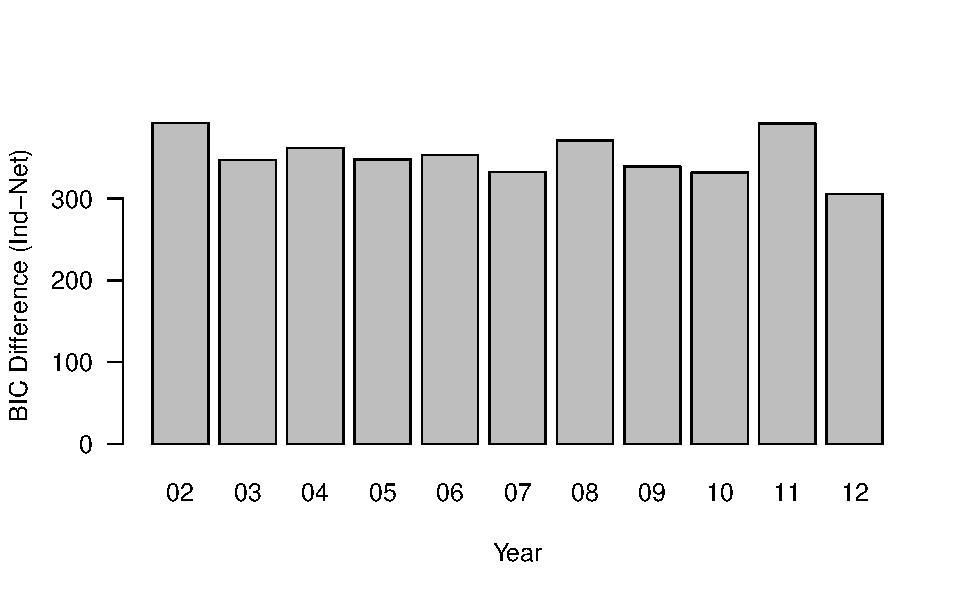
\includegraphics[scale=.6]{slides_figures/BICdiff.pdf}  

%Slide 10
% To evaluate model fit, we subtract the network model BIC from the independent model, meaning that higher numbers indicate better fit. We use BIC since it is robust against increases in model fit simply due to added complexity. Here we see that for every year, inclusion of the network structural dependencies improves model fit.


\end{frame}



\begin{frame}{Count Model and Network Dependencies}

\centering
\begin{tabular}{c@{\hskip -.4cm}c}
\small{Reciprocity} & \small{Transitivity} \\ 
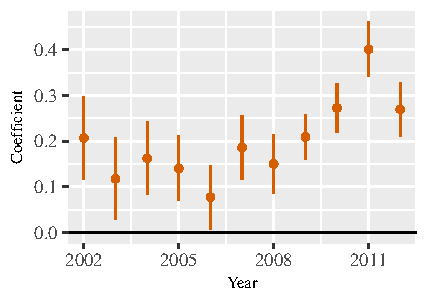
\includegraphics[height=.4\textheight, clip=true, trim=0cm .5cm .1cm .1cm]{slides_figures/rl_plots/Mutuality.pdf}   &
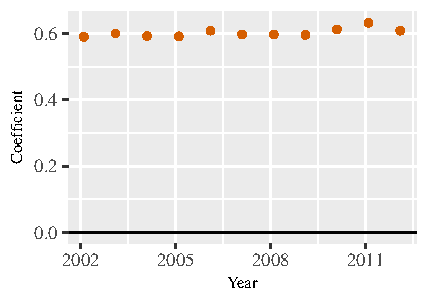
\includegraphics[height=.4\textheight, clip=true, trim=.5cm .5cm .6cm .1cm]{slides_figures/rl_plots/Transitivity.pdf} \\  
\end{tabular}

%Slide 11
% Also, and most important, is that the network terms,  reciprocity and transitivity, are significant and positive , with the bars representing 95% CI, for all years. This supports our hypotheses regarding the network dependencies and demonstrates that models that do not control for these dependencies violate independence assumptions.


\end{frame}


\begin{frame}{Network Statistics}
\centering
  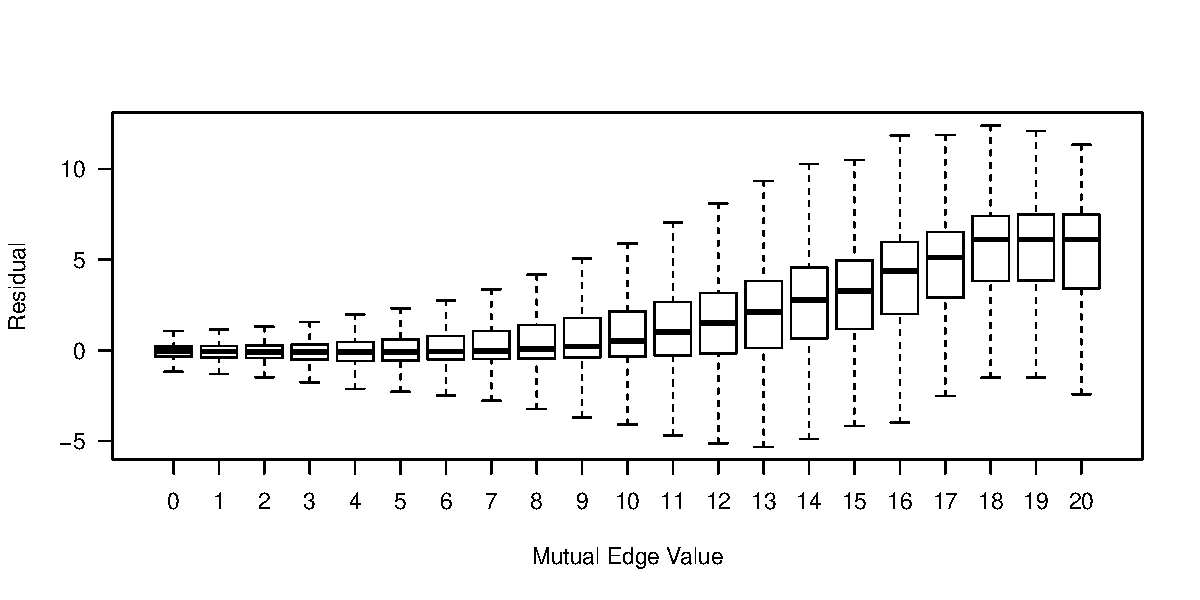
\includegraphics[scale=.45, clip=true, trim=0cm .5cm 0cm 1.9cm]{slides_figures/mutualBoxplot.pdf}\vfill
   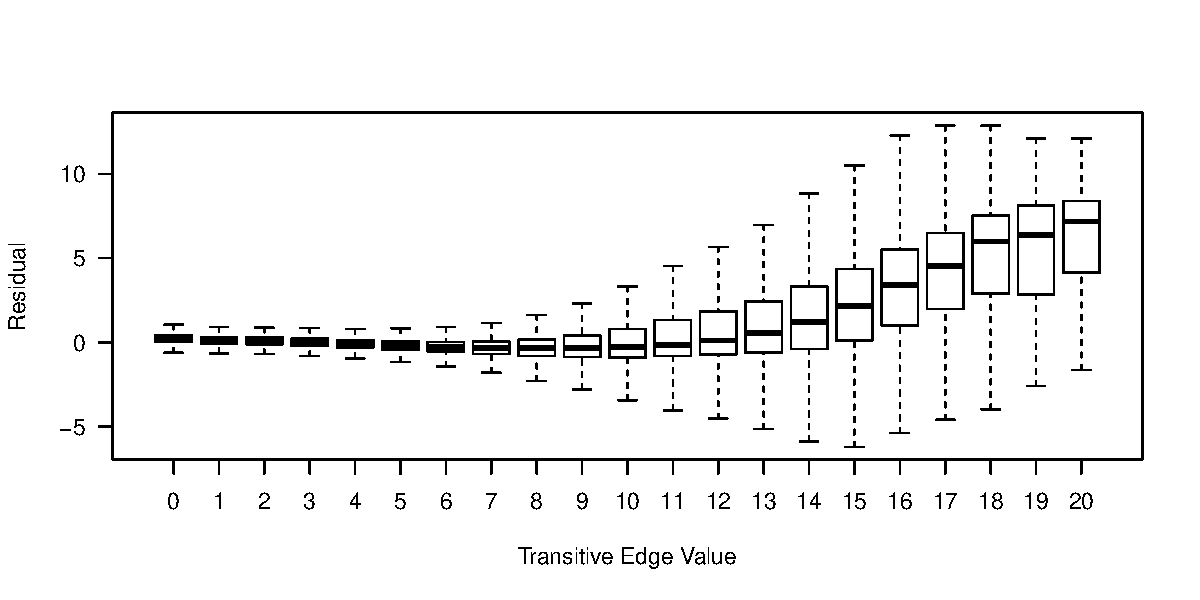
\includegraphics[scale=.45, clip=true, trim=0cm .5cm 0cm 1.9cm]{slides_figures/transitiveBoxplot.pdf}
%Slide 12
% Network statistics are not readily interpreted as OLS coefficients and so plots below provide a way to interpret them. The 'residual' here is the difference between the simulated edge values from the 2012 count ERGM and the value that would be predicted using only the exogenous covariates. And so the mean bar for reciprocity shows the average increase, on the log scale, in addition to that predicted by the exogenous covariates of the FDI from i to j, given a particular increase of the value of j to i. Similarly for transitive edge values, an increase in the highest minimum value of the edge for all the two-paths from i to j, we expect an an average increase in the FDI from i to j.

\end{frame}


\begin{frame}{Covariate Results}

\centering
\begin{tabular}{c@{\hskip -.4cm}c@{\hskip -.4cm}c}
\small{Log-GDP Product} & \small{Distance} & \small{Contiguity} \\
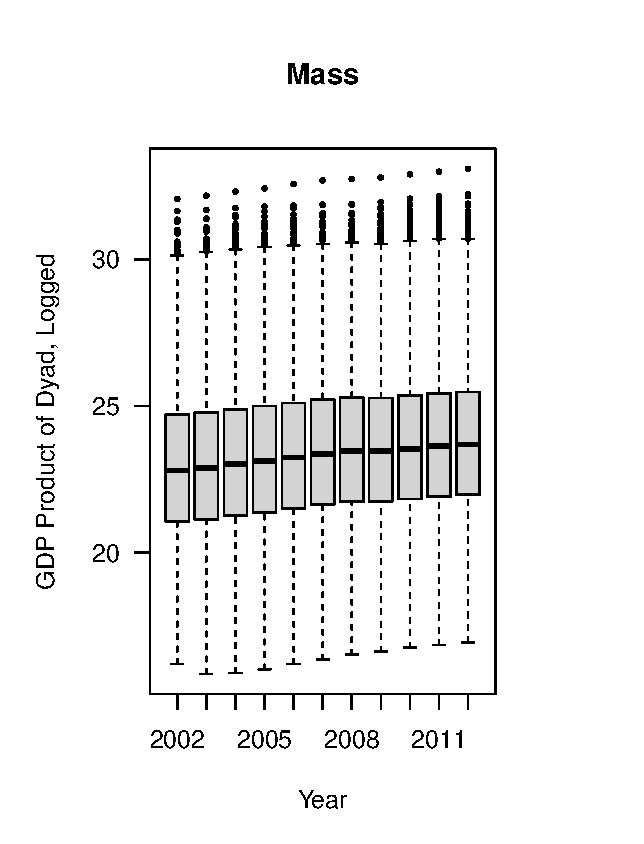
\includegraphics[height=.3\textheight, clip=true, trim=.5cm .5cm 0cm .1cm]{slides_figures/rl_plots/mass.pdf}    &
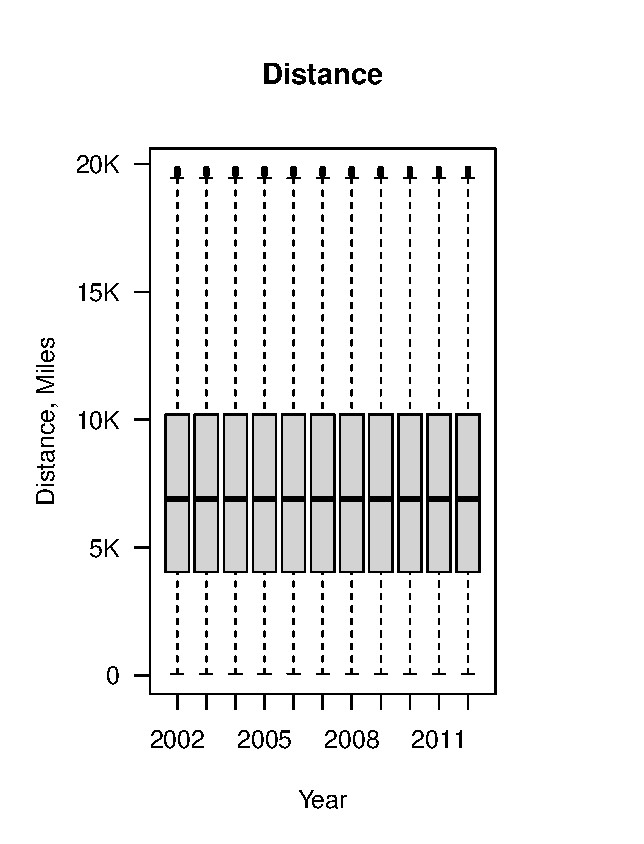
\includegraphics[height=.3\textheight, clip=true, trim=.5cm .5cm 0cm .1cm]{slides_figures/rl_plots/distance.pdf}   &
\includegraphics[height=.3\textheight, clip=true, trim=.5cm .5cm 0cm .1cm]{slides_figures/rl_plots/contiguity.pdf}\\


\small{Dest. Polity} & \small{Dest. Trade Openness} & \small{PTA Depth} \\ 
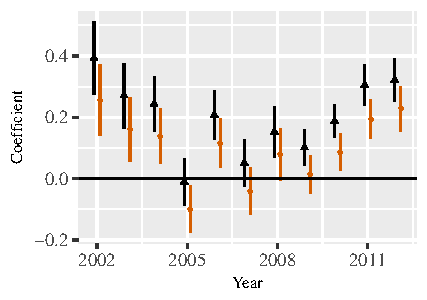
\includegraphics[height=.3\textheight, clip=true, trim=.5cm .5cm 0cm .1cm]{slides_figures/rl_plots/DestPolity.pdf} 
 &
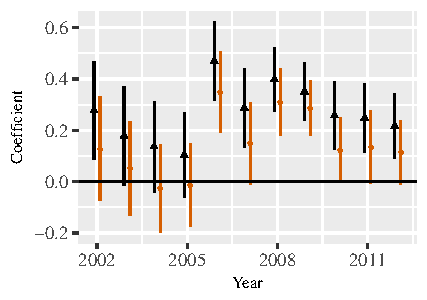
\includegraphics[height=.3\textheight, clip=true, trim=.5cm .5cm 0cm .1cm]{slides_figures/rl_plots/DestTO.pdf}   &
\includegraphics[height=.3\textheight, clip=true, trim=.5cm .5cm 0cm .1cm]{slides_figures/rl_plots/PTAdepth.pdf} \\  
\end{tabular}

%Slide 13
% To illustrate how estimates can be biased, I have included here six of the exogenous covariates from the models, although there were shifts in more than these six. The black points are for models without network dependency controls and the orange points are for the models that include them. We see that the estimates shift in magnitude in the opposite direction and in some instances move from being significant at the 95% level to insignificant. Therefore, by assuming away these dependencies, scholars are in danger of committing Type I errors despite readily available techniques to avoid this pitfall. 

\end{frame}






\begin{frame}{Conclusion and Future Research}

\begin{itemize}
\item{Conclusion}
\begin{itemize}
\item{Network terms are substantively important}
\item{Network terms need to be modeled instead of being assumed away}
\end{itemize}
\item{Future Steps}
\begin{itemize}
\item{Cyclical Weights}
\item{Network dynamics}
\end{itemize}
\end{itemize}

%Slide 14
% To conclude, FDI flows are part of a complex network. The structural dependencies of the network are substantively important and offer insights to scholars attempting to explain the determinants of FDI flows and these dependencies cannot be assumed to be absent even if the scholar is uninterested in explain them. We offer contributions to both of these in this paper.

% The first is including a cyclical weight term to compare the significance between transitive triads and cyclical triads. And second, we plan to adopt variations of the ERGM count model that allow us to account for network dynamics beyond the simple inclusion of the lagged FDI stock level, such as TERGM. Thank you again for allowing me to present here today and I look forward to hearing your suggestions on how this project can be improved.


\end{frame}



\begin{frame}{Additional Covariates}

\centering
\begin{tabular}{c@{\hskip -.4cm}c@{\hskip -.4cm}c}
\small{Sum} & \small{Sum$^{(1/2)}$} & \small{Non-zero} \\
\includegraphics[height=.3\textheight, clip=true, trim=.5cm .5cm 0cm .1cm]{slides_figures/rl_plots/sum.pdf}    &
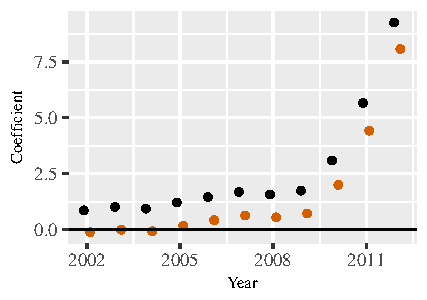
\includegraphics[height=.3\textheight, clip=true, trim=.5cm .5cm 0cm .1cm]{slides_figures/rl_plots/Sum_5.pdf}   &
\includegraphics[height=.3\textheight, clip=true, trim=.5cm .5cm 0cm .1cm]{slides_figures/rl_plots/nonzero.pdf}\\


\small{LDV} & \small{Dest. Political Violence} & \small{Origin Political Violence} \\ 
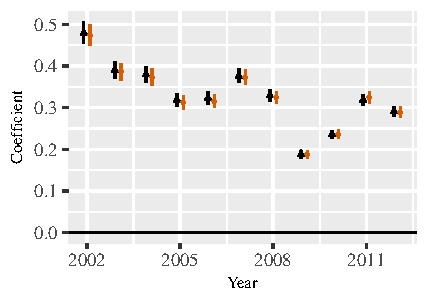
\includegraphics[height=.3\textheight, clip=true, trim=.5cm .5cm 0cm .1cm]{slides_figures/rl_plots/LDV.pdf} 
 &
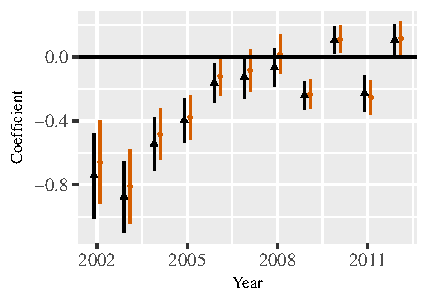
\includegraphics[height=.3\textheight, clip=true, trim=.5cm .5cm 0cm .1cm]{slides_figures/rl_plots/DestPV.pdf}   &
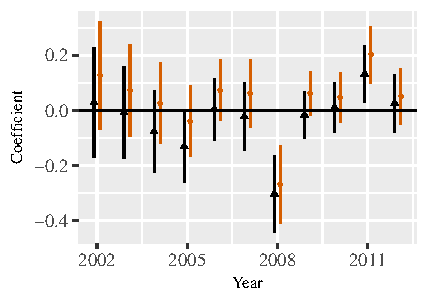
\includegraphics[height=.3\textheight, clip=true, trim=.5cm .5cm 0cm .1cm]{slides_figures/rl_plots/OriginPV.pdf} \\  
\end{tabular}

\end{frame}

\end{document}




